%%%%%%%%%%%%%%%%%%%%%%%%%%%%%%%%%%%%%%%%%
% Short Sectioned Assignment
% LaTeX Template
% Version 1.0 (5/5/12)
%
% This template has been downloaded from:
% http://www.LaTeXTemplates.com
%
% Original author:
% Frits Wenneker (http://www.howtotex.com)
%
% License:
% CC BY-NC-SA 3.0 (http://creativecommons.org/licenses/by-nc-sa/3.0/)
%
%%%%%%%%%%%%%%%%%%%%%%%%%%%%%%%%%%%%%%%%%

%----------------------------------------------------------------------------------------
%	PACKAGES AND OTHER DOCUMENT CONFIGURATIONS
%----------------------------------------------------------------------------------------

\documentclass[paper=a4, fontsize=11pt]{scrartcl} % A4 paper and 11pt font size

\usepackage[T1]{fontenc} % Use 8-bit encoding that has 256 glyphs
\usepackage{fourier} % Use the Adobe Utopia font for the document - comment this line to return to the LaTeX default
\usepackage[english]{babel} % English language/hyphenation
\usepackage{amsmath,amsfonts,amsthm} % Math packages
\usepackage{amssymb}
\newtheorem{theorem}{Claim}
\usepackage{graphicx}
\usepackage{lipsum} % Used for inserting dummy 'Lorem ipsum' text into the template
\usepackage{listings}
\usepackage{fancyvrb} 
\usepackage{bm} 
\usepackage{xcolor} 
\xdefinecolor{gray}{rgb}{0.4,0.4,0.4} 
\definecolor{LightCyan}{rgb}{0.88,1,1}
\xdefinecolor{blue}{RGB}{58,95,205}% R's royalblue3; #3A5FCD
\usepackage{titlesec}
\newcommand{\sectionbreak}{\clearpage}

%\lstset{% setup listings 
%        language=R,% set programming language 
%        basicstyle=\ttfamily\small,% basic font style 
%        keywordstyle=\color{blue},% keyword style 
%        commentstyle=\color{red},% comment style 
%        numbers=left,% display line numbers on the left side 
%        numberstyle=\scriptsize,% use small line numbers 
%        numbersep=10pt,% space between line numbers and code 
%        tabsize=3,% sizes of tabs 
%        showstringspaces=false,% do not replace spaces in strings by a certain character 
%        captionpos=b,% positioning of the caption below 
%        breaklines=true,% automatic line breaking 
%        escapeinside={(*}{*)},% escaping to LaTeX 
%        fancyvrb=true,% verbatim code is typset by listings 
%        extendedchars=false,% prohibit extended chars (chars of codes 128--255) 
%        literate={"}{{\texttt{"}}}1{<-}{{$\bm\leftarrow$}}1{<<-}{{$\bm\twoheadleftarrow$}}1 
%        {~}{{$\bm\sim$}}1{<=}{{$\bm\le$}}1{>=}{{$\bm\ge$}}1{!=}{{$\bm\neq$}}1{^}{{$^{\bm\wedge}$}}1,% item to replace, text, length of chars 
%        alsoletter={.<-},% becomes a letter 
%        alsoother={$},% becomes other 
%        otherkeywords={!=, ~, $, \&, \%/\%, \%*\%, \%\%, <-, <<-, /},% other keywords 
%        deletekeywords={c}% remove keywords 
%} 

\definecolor{listinggray}{gray}{0.9}
\definecolor{lbcolor}{rgb}{0.9,0.9,0.9}
\definecolor{cadmiumgreen}{rgb}{0.0, 0.42, 0.24}
\lstset{
backgroundcolor=\color{lbcolor},
    tabsize=4,    
%   rulecolor=,
    language=[GNU]C++,
        basicstyle=\scriptsize,
        upquote=true,
        aboveskip={1.5\baselineskip},
        columns=fixed,
        showstringspaces=false,
        extendedchars=false,
        breaklines=true,
        prebreak = \raisebox{0ex}[0ex][0ex]{\ensuremath{\hookleftarrow}},
        frame=single,
        numbers=left,
        showtabs=false,
        showspaces=false,
        showstringspaces=false,
        identifierstyle=\ttfamily,
        keywordstyle=\color[rgb]{0,0,1},
        commentstyle=\color[rgb]{0.026,0.112,0.095},
        stringstyle=\color[rgb]{0.627,0.126,0.941},
        numberstyle=\color[rgb]{0.205, 0.142, 0.73},
%        \lstdefinestyle{C++}{language=C++,style=numbers}’.
}
\lstset{
    backgroundcolor=\color{lbcolor},
    tabsize=4,
  language=C++,
  captionpos=b,
  tabsize=3,
  frame=lines,
  numbers=left,
  numberstyle=\tiny,
  numbersep=5pt,
  breaklines=true,
  showstringspaces=false,
  basicstyle=\footnotesize,
%  identifierstyle=\color{magenta},
  keywordstyle=\color[rgb]{0,0,1},
  commentstyle=\color{cadmiumgreen},
  stringstyle=\color{red}
  }

\usepackage{sectsty} % Allows customizing section commands
%\usepackage[left=2cm,right=2cm,top=2cm,bottom=3cm]{geometry}
\usepackage[margin=1in]{geometry}
\addtolength{\topmargin}{-.1in}
\allsectionsfont{\normalfont\scshape} % Make all sections centered, the default font and small caps

\usepackage{fancyhdr} % Custom headers and footers
\pagestyle{fancyplain} % Makes all pages in the document conform to the custom headers and footers
\fancyhead{} % No page header - if you want one, create it in the same way as the footers below
\fancyfoot[L]{} % Empty left footer
\fancyfoot[C]{} % Empty center footer
\fancyfoot[R]{\thepage} % Page numbering for right footer
\renewcommand{\headrulewidth}{0pt} % Remove header underlines
\renewcommand{\footrulewidth}{0pt} % Remove footer underlines
\setlength{\headheight}{2pt} % Customize the height of the header

\numberwithin{equation}{section} % Number equations within sections (i.e. 1.1, 1.2, 2.1, 2.2 instead of 1, 2, 3, 4)
\numberwithin{figure}{section} % Number figures within sections (i.e. 1.1, 1.2, 2.1, 2.2 instead of 1, 2, 3, 4)
\numberwithin{table}{section} % Number tables within sections (i.e. 1.1, 1.2, 2.1, 2.2 instead of 1, 2, 3, 4)

\setlength\parindent{0pt} % Removes all indentation from paragraphs - comment this line for an assignment with lots of text

%----------------------------------------------------------------------------------------
%	TITLE SECTION
%----------------------------------------------------------------------------------------

\newcommand{\horrule}[1]{\rule{\linewidth}{#1}} % Create horizontal rule command with 1 argument of height

\title{	
\normalfont \normalsize 
\textsc{University of Texas} \\ [25pt] % Your university, school and/or department name(s)
\horrule{0.1pt} \\[.5cm] % Thin top horizontal rule
\huge Peer review: Jennifer Starling \\ % The assignment title
\horrule{.1pt} \\[0cm] % Thick bottom horizontal rule
}
\vspace{10mm}
\subtitle{SDS 385}

\author{David Puelz} % Your name

\date{\normalsize\today} % Today's date or a custom date

\begin{document}
\maketitle
\tableofcontents
\newpage


%----------------------------------------------------------------------------------------
%	PROBLEM 1
%----------------------------------------------------------------------------------------

\section{Comments on code}

I enjoyed reading through your work and code.  It is very well-documented and easy to understand. Your understanding of the statistics in class is rock-solid, and your efforts on the assignments are tremendous (do I sound like Donald Trump?).  I have no specific suggestions other than to continue to modularize your code (both Cpp and R) as much as possible.  By having everything in functions, you can do so much with relatively little effort and the code becomes easy to debug.

\section{Cross-validation exercise}

I was most interested in comparing our cross-validation approaches.  To do so, I modified your Cpp function to allow for training and testing the model after several passes of stochastic gradient descent.  I removed some of your original comments and added some additional lines of code at the very beginning and end -- I tried not to touch anything else!  The first ``train" observations of X are used to train the model, and the remaining observations are used to test the model.
\\
\\
Let me know if you have any questions regarding my modifications.  I'll post the code on github as well. 

\begin{lstlisting}
List sparse_sgd_logit(MapMatd Xtall, VectorXd Y, VectorXd m, double step, int train, int npass, VectorXd beta0, float lambda){

// David modified here for Cpp cross-validation
// Training and test X!
int totalcols = Xtall.cols();
DaveMat X = Xtall.leftCols(train);
DaveMat Xtest = Xtall.rightCols(totalcols-train);
int nSamptest = Xtest.cols();

//-----------------------------------
//INITIALIZE VALUES:
int p = X.rows(); 		//Number of features in X matrix.
int n = X.cols(); 		//Number of observations in X matrix.
int iter = 0;			//Global iteraton counter.
int j = 0;				//Inner iterator row number.
double epsilon = 1E-6;	//Constant for Adagrad numeric stability.

//Initialize vectors for beta, gradient, and doubles for Adagrad updates in sparse row loop.
VectorXd beta_hat(p);			//Beta_hat vector, length p.
beta_hat = beta0;				//Set beta_hat to initial beta input value.
VectorXd hist_grad(p);		//Vector to hold running hist_grad.  Will be updated piecewise in Sparse Row Loop.
VectorXd adj_grad(p);		//Vector to hold adj_grad_j for each beta_hat_j.

//Initialize hist_grad values at 1E-3 for numerical stability.
for (int i=0;i<p;i++){
hist_grad(i) = 1E-3;
adj_grad(i) = 0;
}

double grad_j = 0;				//Holds jth element of gradient.  Do not need to store whole gradient at once.
//double adj_grad_j = 0;			//Holds jth element of adj_grad for Adagrad.  (In Sparse Row Loop)

//Initialize elements to hold X, Y and m for a single observation (column).
SparseVector<double> Xi(n);
Xi=X.innerVector(0);

double Yi = Y(0);
double mi = m(0);
double wi = .5;			//wi will be a scalar, since calculating weights in inner vector.
double wi_exponent = 0;	//Holds the exponential part of the wi update.

//Initialize vector (length p) to keep track of when each predictor updated, for lazy updates.
NumericVector last_updated(p,0.0);
double skip = 1;	//Holds how many iterations since last update for a j row of ith col.

//Initialize vectors to hold log-likelihood and running avg neg log-likelihood.
double nll = 0;								//Holds avg neg loglikelihood for the current i obs.	
NumericVector nll_ra(n*npass,0.0);			//Stores running avg loglikelihood.

//Initialize variable to hold accumulated penalty for a beta_j.
double accum_l2_penalty = 0;	//Holds accumulated penalty.
double gam = 0;					//Holds step*adj_grad_j, for use in calculating accumulated penalty.

//-----------------------------------
//LOOPING THROUGH DATA SET:

//Loop 1: Loop over entire data set npass times.
for (int np=0; np < npass; ++np){

//Rcpp::Rcout << "npass:" << np << std::endl; //REMOVE LATER: Output start of each npass through data to R console.

//Loop 2:  Loop through observations (cols) of X data set.
for (int i=0; i<n; ++i){

//Set up the single observation for the next stochastic iteration.  
Xi = X.innerVector(i);	//Select new X observation; the ith column of matrix X.
Yi = Y(i);				//Select new Y observation; the ith value of vector Y.
mi = m(i);				//Select new m observation; the ith value of sample size vector m.			

//Update wi probability value.  (w is scalar, since looking at one obs.)
wi_exponent = Xi.dot(beta_hat); //breaking out exponential term helps with efficiency.
wi = 1 / (1 + exp(-wi_exponent));

//Update neg loglikelihood and running average.
nll = -(Yi * log(wi + epsilon) + (mi - Yi) * log(1 - wi + epsilon));
if(iter > 0) {
nll_ra(iter) = (nll_ra(iter-1) * (iter-1) + nll) / iter;
}			

//Loop 3: Loop through active feature values (rows) of X data set for ith obs (col).
for (InIterVec it(Xi); it; ++it){

//Set j to the feature (row) number.
j = it.index();

//--------------------------------
//STEP 1: Part 1 of Row Updates for ith Feature:  Deferred (lazy) L2 penalty updates.
//This aggregates all of the penalty-only updates since last time a feature was updated.
//"Penalty-only" updates refers to the gradient not being updated except
//for adding the 2*lambda*beta penalty term.

//Cap maximum number of recursive updates at 5, for numeric stability.
//This works bc updates go to zero fairly quickly when lambda<1.
skip = iter - last_updated(j);	//Number of iters since last update. (Skip=1 means updated last iter.)
if (skip > 5){  skip = 5;}		
last_updated(j) = iter;			//Update the last_updated flag for all j's active in this iter.

//Calculate accum penalty.  Based on recursion defined in my notes.
//NOTE: This is the gradient for minimizing the neg log-lhood.  
//See final note in recursion doc.
gam = step*adj_grad(j);
accum_l2_penalty = beta_hat(j) * ( (1 - pow(1+lambda*gam,skip)) / (1-lambda*gam) );

//Add accum l2 penalty to beta_hat_j before doing current iteration update.
beta_hat(j) -= accum_l2_penalty; 

//--------------------------------
  //STEP 2: Continue with updates for jth row in ith col.

//Calculate l2 norm penalty.
double l2penalty = 2*lambda*beta_hat(j);

//Update the jth gradient term.  Note: it.value() looks up Xji for nonzero entries.
grad_j = (mi*wi-Yi) * it.value() + l2penalty;  

//Update the jth hist_grad term for Adagrad.  
//This is the running total of the jth squared gradient term.
hist_grad(j) += grad_j * grad_j;

//Calculate the jth adj_grad term for Adagrad.
adj_grad(j) = grad_j * invSqrt(hist_grad(j) + epsilon);

//Calculate the updated jth beta_hat term.
beta_hat(j) -= step*adj_grad(j);	
}			
++iter; //Update global counter.  (Counts each iteration.)
} //End Loop 2: Loop through observations (cols) of X data set.	
} //End Loop 1: Loop over entire data set npass times.

//-----------------------------------
  //Loop 4: Loop over predictors to catch any last accumulated penalty updates
//for predictors not updated in last iteration.
for (int j=0; j<p; ++j){
  //Using (iter-1) since last_updated indexes from 0, and n is based on counting rows from 1.
  skip = (iter-1) - last_updated(j); 
  
  //Cap maximum number of recursive updates at 5, for numeric stability.
  //This works bc updates go to zero fairly quickly when lambda<1.	
  if (skip > 5){  skip = 5;}			
  
  //Calculate accum penalty.
  gam = step*adj_grad(j);	
  accum_l2_penalty = beta_hat(j) * ( (1 - pow(1+lambda*gam,skip)) / (1-lambda*gam) );
  
  //Update beta_j's to add accum penalty.
  beta_hat(j) -= accum_l2_penalty; 
}	


// Now, the big loop to test
double tally = 0;
double tally2 = 0;
double tally3 = 0;
double num1s = 0;
double num0s = 0;
int yhat;
for(int i = 0; i < nSamptest; i++)
{
  SpVec Xsamp = Xtest.col(i);
  double XB = Xsamp.dot(beta_hat);
  double w = 1 / (1 + exp(-XB));
  double y = Y(i+train);
  
  if(w < 0.5)
  {
    yhat = 0;
    if(y==0){ tally3 += 1; }
  }
  else
  {
    yhat = 1;
    if(y==1){ tally2 += 1; }
  }
  tally += fabs(y-yhat);
  if(y==0){ num0s += 1; }
  else{ num1s +=1; }
}
double classrate = 1 - (tally/nSamptest);
double sensi = (tally2/num1s); 
double speci = (tally3/num0s); 

  
  //-----------------------------------
  //Return function values.
  return Rcpp::List::create(
  _["n"] = n,
  _["p"] = p,
  _["iter"] = iter,
  _["beta_hat"] = beta_hat,
  _["classrate"] = classrate
  ) ;
  
}
\end{lstlisting}

\newpage
\subsection{Comparing the solution paths}

I ran your code as well as mine, choosing the first 80\% of the observations as training data and the remaining 20\% as testing data.  In each case, the X matrix is scaled the same way.  I ran the algorithm 10 passes through the training data and for 20 different $\lambda$ values.  The results are shown in the plot below.

\begin{figure}[h]
\centering
	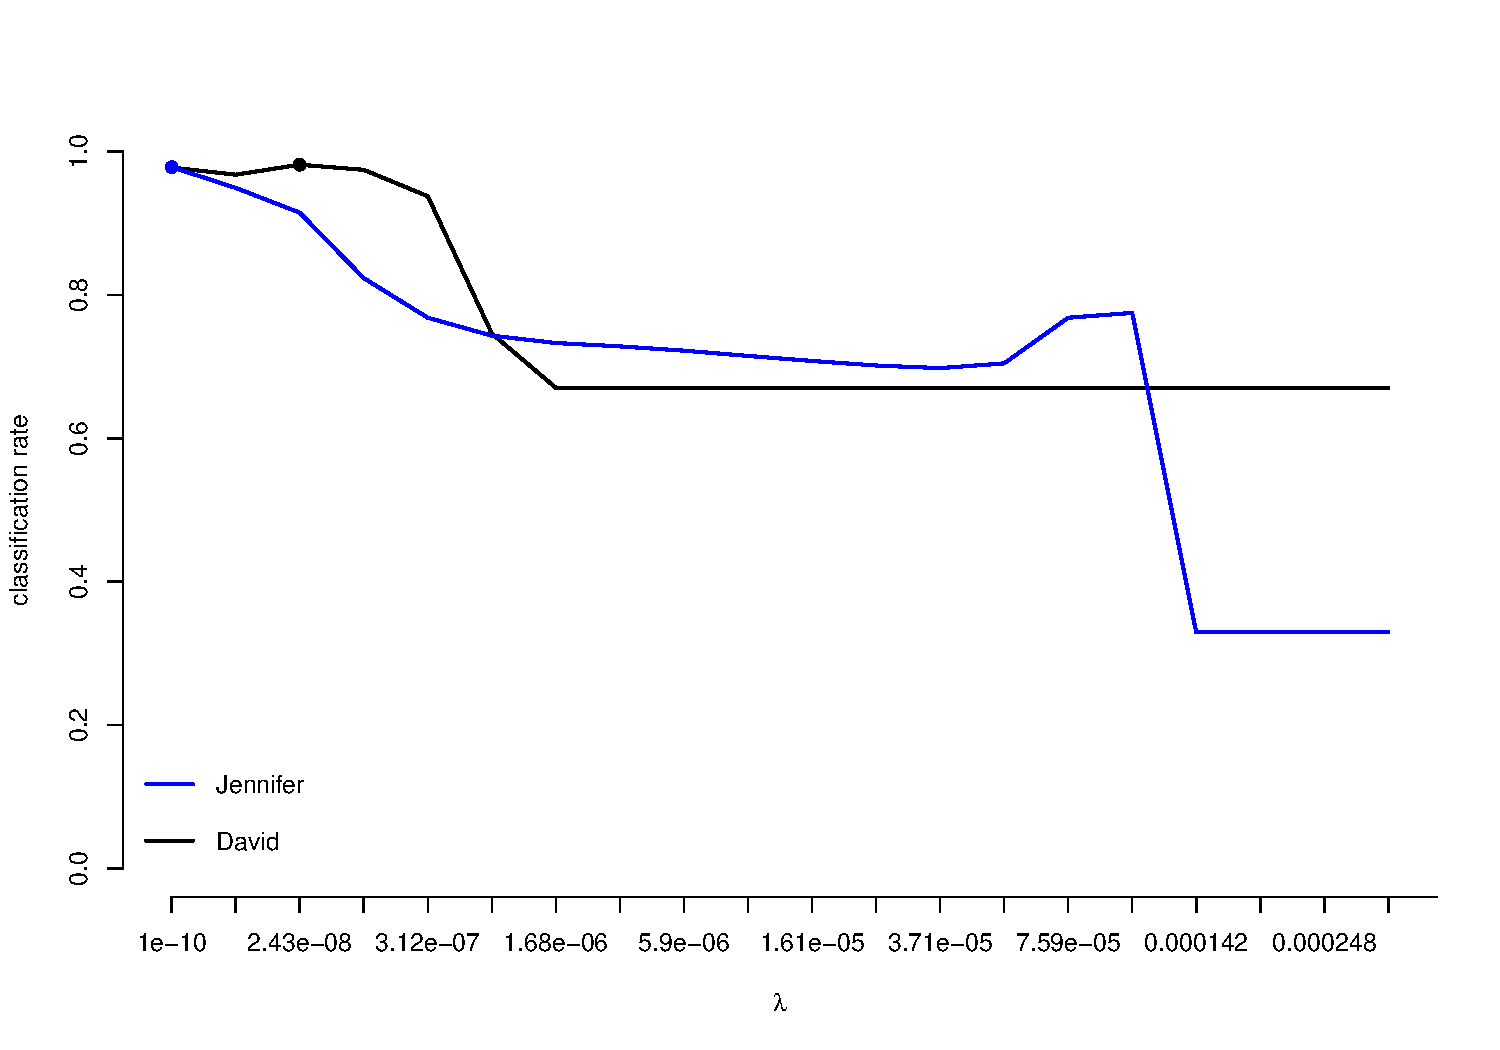
\includegraphics[scale=0.62]{SolutionPathCompare}\caption{Solution paths for our two implementations of SGD}
\end{figure}

The dots identify the maximum classification rate for the trained model on the testing data.  I find the differences interesting, and I believe we differ in our updating of the penalties.  This could potentially result in the $\lambda$'s having different impacts on the models' out-of-sample performance. Kind of interesting!


\end{document}